% LaTeX support: latex@mdpi.com 
% In case you need support, please attach all files that are necessary for compiling as well as the log file, and specify the details of your LaTeX setup (which operating system and LaTeX version / tools you are using).

% You need to save the "mdpi.cls" and "mdpi.bst" files into the same folder as this template file.

%=================================================================
\documentclass[ijgi,article,submit,moreauthors,pdftex,10pt,a4paper]{Definitions/mdpi} 
\usepackage{subfig}

% If you would like to post an early version of this manuscript as a preprint, you may use preprint as the journal and change 'submit' to 'accept'. The document class line would be, e.g. \documentclass[preprints,article,accept,moreauthors,pdftex,10pt,a4paper]{mdpi}. This is especially recommended for submission to arXiv, where line numbers should be removed before posting. For preprints.org, the editorial staff will make this change immediately prior to posting.

%
%--------------------
% Class Options:
%--------------------
% journal
%----------
% Choose between the following MDPI journals:
% acoustics, actuators, addictions, admsci, aerospace, agriculture, agronomy, algorithms, animals, antibiotics, antibodies, antioxidants, applsci, arts, asi, atmosphere, atoms, axioms, batteries, bdcc, behavsci, beverages, bioengineering, biology, biomedicines, biomimetics, biomolecules, biosensors, brainsci, buildings, carbon, cancers, catalysts, cells, ceramics, challenges, chemengineering, chemosensors, children, cleantechnol, climate, clockssleep, cmd, coatings, colloids, computation, computers, condensedmatter, cosmetics, cryptography, crystals, cybersecurity, data, dentistry, designs, diagnostics, dairy, diseases, diversity, drones, econometrics, economies, education, electrochem, electrochemistry, electronics, energies, entropy, environments, epigenomes, est, fermentation, fibers, fire, fishes, fluids, foods, forecasting, forests, fractalfract, futureinternet, galaxies, games, gastrointestdisord, gels, genealogy, genes, geohazards, geosciences, geriatrics, hazardousmatters, healthcare, heritage, highthroughput, horticulturae, humanities, hydrology, informatics, information, infrastructures, inorganics, insects, instruments, ijerph, ijfs, ijms, ijgi, ijtpp, inventions, j, jcdd, jcm, jcs, jdb, jfb, jfmk, jimaging, jof, jintelligence, jlpea, jmmp, jmse, jpm, jrfm, jsan, land, languages, laws, life, literature, logistics, lubricants, machines, magnetochemistry, make, marinedrugs, materials, mathematics, mca, medsci, medicina, medicines, membranes, metabolites, metals, microarrays, micromachines, microorganisms, minerals, modelling, molbank, molecules, mps, mti, nanomaterials, ncrna, neonatalscreening, neuroglia, nitrogen, nutrients, ohbm, particles, pathogens, pharmaceuticals, pharmaceutics, pharmacy, philosophies, photonics, plants, plasma, polymers, polysaccharides, proceedings, processes, proteomes, publications, quaternary, qubs, reactions, recycling, religions, remotesensing, reports, resources, risks, robotics, safety, sci, scipharm, sensors, separations, sexes, sinusitis, smartcities, socsci, societies, soilsystems, sports, standards, stats, surfaces, surgeries, sustainability, symmetry, systems, technologies, toxics, toxins, tropicalmed, universe, urbansci, vaccines, vehicles, vetsci, vibration, viruses, vision, water, wem, wevj
%---------
% article
%---------
% The default type of manuscript is article, but can be replaced by: 
% abstract, addendum, article, benchmark, book, bookreview, briefreport, casereport, changes, comment, commentary, communication, conceptpaper, correction, conferenceproceedings, conferencereport, expressionofconcern, meetingreport, creative, datadescriptor, discussion, editorial, essay, erratum, hypothesis, interestingimages, letter, meetingreport, newbookreceived, opinion, obituary, projectreport, reply, reprint, retraction, review, perspective, protocol, shortnote, supfile, technicalnote, viewpoint
% supfile = supplementary materials
% protocol: If you are preparing a "Protocol" paper, please refer to http://www.mdpi.com/journal/mps/instructions for details on its expected structure and content.
%----------
% submit
%----------
% The class option "submit" will be changed to "accept" by the Editorial Office when the paper is accepted. This will only make changes to the frontpage (e.g. the logo of the journal will get visible), the headings, and the copyright information. Also, line numbering will be removed. Journal info and pagination for accepted papers will also be assigned by the Editorial Office.
%------------------
% moreauthors
%------------------
% If there is only one author the class option oneauthor should be used. Otherwise use the class option moreauthors.
%---------
% pdftex
%---------
% The option pdftex is for use with pdfLaTeX. If eps figures are used, remove the option pdftex and use LaTeX and dvi2pdf.

%=================================================================
\firstpage{1} 
\makeatletter 
\setcounter{page}{\@firstpage} 
\makeatother
\pubvolume{xx}
\issuenum{1}
\articlenumber{1}
\pubyear{2018}
\copyrightyear{2018}
\externaleditor{Academic Editor: name}
\history{Received: date; Accepted: date; Published: date}
%\updates{yes} % If there is an update available, un-comment this line

%------------------------------------------------------------------
% The following line should be uncommented if the LaTeX file is uploaded to arXiv.org
%\pdfoutput=1

%=================================================================
% Add packages and commands here. The following packages are loaded in our class file: fontenc, calc, indentfirst, fancyhdr, graphicx, lastpage, ifthen, lineno, float, amsmath, setspace, enumitem, mathpazo, booktabs, titlesec, etoolbox, amsthm, hyphenat, natbib, hyperref, footmisc, geometry, caption, url, mdframed, tabto, soul, multirow, microtype, tikz

%=================================================================
%% Please use the following mathematics environments: Theorem, Lemma, Corollary, Proposition, Characterization, Property, Problem, Example, ExamplesandDefinitions, Hypothesis, Remark, Definition
%% For proofs, please use the proof environment (the amsthm package is loaded by the MDPI class).

%=================================================================
% Full title of the paper (Capitalized)
\Title{Dataset Reduction Techniques to Speed Up SVD Analyses}

% Author Orchid ID: enter ID or remove command
\newcommand{\orcidauthorA}{0000-0002-7712-6627} % Add \orcidA{} behind the author's name
\newcommand{\orcidauthorB}{0000-0003-2225-1428} % Add \orcidB{} behind the author's name
\newcommand{\orcidauthorC}{0000-0002-1769-6310} % Add \orcidC{} behind the author's name

% Authors, for the paper (add full first names)
\Author{Laurens Bogaardt $^{1}$\orcidA{}, Romulo Goncalves $^{1}$\orcidB{}, Raul Zurita-Milla $^{2,}$*\orcidC{} and Emma Izquierdo-Verdiguier $^{3}$}

% Authors, for metadata in PDF
\AuthorNames{Laurens Bogaardt, Romulo Goncalves, Raul Zurita-Milla, Emma Izquierdo-Verdiguier}

% Affiliations / Addresses (Add [1] after \address if there is only one affiliation.)
\address{%
$^{1}$ \quad Netherlands eScience Center; l.bogaardt@esciencecenter.nl, r.goncalves@esciencecenter.nl\\
$^{2}$ \quad Faculty ITC, University of Twente; r.zurita-milla@utwente.nl\\
$^{3}$ \quad IPL, Universitat de Valencia; emma.izquierdo@uv.es}

% Contact information of the corresponding author
\corres{Correspondence: r.zurita-milla@utwente.nl}

% Current address and/or shared authorship
%\firstnote{Current address: Affiliation 3} 
%\secondnote{These authors contributed equally to this work.}
% The commands \thirdnote{} till \eighthnote{} are available for further notes

% Simple summary
%\simplesumm{}

%\conference{} % An extended version of a conference paper

% Abstract (Do not insert blank lines, i.e. \\) 
\abstract{Performing SVD analyses on large datasets can be computationally costly and time consuming. Often, techniques exist to arrive at the same output, or at a close approximation, which require far less effort. This article examines several such techniques in combination with the inherent scale of the structure within the data. When the values of a dataset vary slowly, e.g. in a spatial field of temperature over a country, the field contains large scale structure and there is a high level of autocorrelation. Hence, datasets do not need a high resolution to describe such fields. Using generated Gaussian Random Fields with various levels of autocorrelation, we examine rank decomposition, coarsening and approximate SVD procedures to study their accuracy for different levels of autocorellation. As the main result, this article provides researchers with a decision tree indicating which technique to use when and predicting the resulting level of accuracy based on the dataset's structure scale. Finally, these techniques and predictions, based on simulated data, are verified using real-world geospatial datasets.}

% Keywords
\keyword{Singular value decomposition, autocorrelation, rank deficiency, data reduction, coarsening, approximate SVD, Gaussian Random Fields}

% The fields PACS, MSC, and JEL may be left empty or commented out if not applicable
%\PACS{J0101}
%\MSC{}
%\JEL{}

%%%%%%%%%%%%%%%%%%%%%%%%%%%%%%%%%%%%%%%%%%
% Only for the journal Applied Sciences:
%\featuredapplication{Authors are encouraged to provide a concise description of the specific application or a potential application of the work. This section is not mandatory.}
%%%%%%%%%%%%%%%%%%%%%%%%%%%%%%%%%%%%%%%%%%

%%%%%%%%%%%%%%%%%%%%%%%%%%%%%%%%%%%%%%%%%%
% Only for the journal Data:
%\dataset{DOI number or link to the deposited data set in cases where the data set is published or set to be published separately. If the data set is submitted and will be published as a supplement to this paper in the journal Data, this field will be filled by the editors of the journal. In this case, please make sure to submit the data set as a supplement when entering your manuscript into our manuscript editorial system.}

%\datasetlicense{license under which the data set is made available (CC0, CC-BY, CC-BY-SA, CC-BY-NC, etc.)}

%%%%%%%%%%%%%%%%%%%%%%%%%%%%%%%%%%%%%%%%%%
% Only for the journal Toxins
%\keycontribution{The breakthroughs or highlights of the manuscript. Authors can write one or two sentences to describe the most important part of the paper.}

%\setcounter{secnumdepth}{4}
%%%%%%%%%%%%%%%%%%%%%%%%%%%%%%%%%%%%%%%%%%
\begin{document}
%%%%%%%%%%%%%%%%%%%%%%%%%%%%%%%%%%%%%%%%%%
%% Only for the journal Gels: Please place the Experimental Section after the Conclusions

%%%%%%%%%%%%%%%%%%%%%%%%%%%%%%%%%%%%%%%%%%
%\setcounter{section}{-1} %% Remove this when starting to work on the template.
%\section{How to Use this Template}
%The template details the sections that can be used in a manuscript. Note that the order and names of article sections may differ from the requirements of the journal (e.g. the positioning of the Materials and Methods section). Please check the instructions for authors page of the journal to verify the correct order and names. For any questions, please contact the editorial office of the journal or support@mdpi.com. For LaTeX related questions please contact Janine Daum at latex-support@mdpi.com.
%The order of the section titles is: Introduction, Materials and Methods, Results, Discussion, Conclusions for these journals: aerospace,algorithms,antibodies,antioxidants,atmosphere,axioms,biomedicines,carbon,crystals,designs,diagnostics,environments,fermentation,fluids,forests,fractalfract,informatics,information,inventions,jfmk,jrfm,lubricants,neonatalscreening,neuroglia,particles,pharmaceutics,polymers,processes,technologies,viruses,vision

\section{Introduction}
\label{sec:Introduction}

%The introduction should briefly place the study in a broad context and highlight why it is important. It should define the purpose of the work and its significance. The current state of the research field should be reviewed carefully and key publications cited. Please highlight controversial and diverging hypotheses when necessary. Finally, briefly mention the main aim of the work and highlight the principal conclusions. As far as possible, please keep the introduction comprehensible to scientists outside your particular field of research. Citing a journal paper \cite{ref-journal}. And now citing a book reference \cite{ref-book}. Please use the command \citep{ref-journal} for the following MDPI journals, which use author-date citation: Administrative Sciences, Arts, Econometrics, Economies, Genealogy, Humanities, IJFS, JRFM, Languages, Laws, Religions, Risks, Social Sciences.

Singular Value Decomposition (SVD) analysis when applied to a single spatial field helps to identify areas that behave similarly. In many real-world applications, however, the analysis of a field does not only involve a single time period but includes data over multiple weeks, months or years. Researchers typically compare two such datasets using \textit{Maximum Covariance Analysis} (MCA) and \textit{Canonical Correlation Analysis} (CCA) to find patterns which occur frequently and simultaneously~\cite{Eshel2011, Storch1999}. Such a pattern, or mode, is a combination of a row- and a column basis vector. One technique to determine these modes is to perform an SVD on the product of the standardised datasets. In some domains, the term SVD is used synonymously with MCA. In an MCA, modes are found where the row- and the column vector covary maximally, whereas in a CCA, they correlate maximally~\cite{Bretherton1992}.

Performing \textit{Singular Value Decompositions} (SVD's) on large datasets can be computationally costly and time consuming [RG: Let's find this facebook article about an expensive computation of SVD.]. Often, techniques exist to arrive at the same output, or at a close approximation, which require far less effort. This article studies several procedures which exploit autocorrelation and rank decomposition to analyse data in an efficient manner. To the best of our knowledge, it is the first thoral study in GeoSciences using large-data sets~\cite{Golub1970, Bjorck1973, Chan1982}. In this article, we outline when certain techniques are useful and we make predictions about the error incurred in the approximations based on the level of autocorrelation of the input data.

To arrive at these predictions, \textit{Gaussian Random Fields} (GRF's) are generated with various levels of autocorrelation and are subsequently reduced in size. The amount of error incurred in this reduction is determined by comparing the SVD of the reduced dataset to that of the original. Finally, the techniques and predictions, based on simulated data, are verified using real-world geospatial datasets. The reported results come from calculations performed in an accompanying \textit{Jupyter Notebook} which can be found in the online supplementary material~\cite{Bogaardt2018}. In order to develop intuition, some matrix algebra is briefly reviewed first, followed by discussion on the data characteristics of some data sets use in GeoSciences.

%Maybe rename it to rank deficiency to explain what it is and how it reduces storage and number of vector computations.
\subsection{Matrix decomposition}
\label{sec:Introduction/Matrix decompostion}

Data sets with two or more dimensions can be represented by a matrix; for instance, a group of~$n$ individuals who report scores on~$m$ questions or the temperatures at~$m$ locations measured over~$n$ time periods. These values can be arranged in a matrix with~$m$ rows and~$n$ columns. Like a vector, a matrix is a combination of basis vectors which indicate direction, each with a coefficient which indicates magnitude. As an extension of the vector, a matrix has two bases, the row- and the column basis, which can also be changed via a rotation. A clever basis to rotate into is one where the product of the first row- and column basis vectors explains as much of the variance in the dataset as possible. Subsequent pairs of basis vectors, known as \textit{modes}, explain as much of the remaining variance as possible while being orthogonal to all previous modes. Such basis vectors are called \textit{Principle Components} (PC's) or \textit{Empirical Orthogonal Functions} (EOF's) and they are found via an SVD of the matrix.

If there exists a rotation for which some coefficients become zero, the matrix needs fewer basis vectors to describe it than are available. In a sense, it is underdetermined; its internal dimension is smaller than what would be expected from its $m$~by~$n$ size. This is the concept of matrix \textit{rank}; if the rows and columns both span a subspace of dimension~$r$, a matrix has rank~$r$. A matrix is said to have full rank if $r = \text{min}(m, n)$, the maximum number of linearly independent basis vectors, and rank deficient if $r < \text{min}(m, n)$. 

An SVD is a special type of rank decomposition which results in a set of orthonormal column basis vectors $U$, a list of coefficients $s$ and a set of row basis vectors $V$. For rank deficient matrices, some of the coefficients, known as singular values, are zero. Hence, a rank decomposed version of the original data is used to reduce the storage and computational requirements for a SVD analysis. A rank decomposition or factorization is the splitting of a matrix into a product where each factor has full rank. For example, an $m$ by $n$ matrix of rank $r$ can be decomposed into an $m$ by $r$ matrix multiplied by an $r$ by $n$ one. Thus, instead of the entire, original dataset, which requires $m \times n$ units of storage and computing the product with a vector requires $m \times n$ flops, it is possible to use the rank decomposed version to reduce storage and have faster computations. The rank decomposed version requires $m \times r + r \times n$ units of storage and an equal number of flops for the vector multiplication~\cite{Martinsson2016}. If $r$ is small, this can be a substantial improvement. 

\subsection{Data characteristics}
Real-world data are gathered by machines with finite precision, therefore, the mathematical rank $r$ of a dataset is usually not relevant~\cite{Martinsson2016}. This means that the \textit{information} contained in the data is limited by the noise level. Even though some singular values of a dataset are not zero, they may be small enough to be considered noise. Without losing much information, we can approximate a dataset by another matrix of rank $l$, with $l < r$. An approximation of the original data set with a matrix of rank~$l$ will be enough to identify areas that behave similarly, i.e., it may not be necessary to determine the mathematically exact SVD. 

Following the Eckart-Young theorem, the best approximation is one described in the same bases as the original dataset, taking a subset of the $l$ largest singular values and truncating the remainder~\cite{Eckart1936}. Setting a threshold~$\epsilon$, the dataset is the approximate rank deficient if some singular values fall below~$\epsilon$. Then, it has an $\epsilon$-rank of $l$ and the spectral norm of the difference with its approximation is at most~$\epsilon$~\cite{Martinsson2016}. The idea is to reduce the data to the point where the error due to reduction is around the noise level. 

Beside the irrevelant information, there is also data redundancy. In domains such as climate science, datasets are typically spatio-temporal fields e.g. of global temperatures. In such fields, values vary slowly and neighbouring points are not entirely independent of one another, neither in space nor in time~\cite{Eshel2011}. Then, there is a high level of autocorrelation and the field contains large scale structure. Such redundancy in the data means the matrix is rank deficient. Through syntetic spatio-temporal fields with different levels of autocorrelation we study the precision of different SVD implementations.

%\subsection{Efficiency}
%\label{sec:Introduction/Efficiency}
%
%The term \textit{efficiency} used in this article is related to the concept of rank deficiency. A calculation is called efficient if it never requires the construction of an unnecessarily large, intermediate matrix. The best way to build up intuition for this concept is via an example.
%
%One often wants to find the norm of the difference between two fields. This can be achieved directly by subtracting one matrix from the other and summing the square of the elements. However, for large matrices, the direct calculation may be unnecessarily time consuming. Let's assume datasets~$A$ and~$B$ are rank deficient and stored in SVD form. As discussed in section~\ref{sec:Introduction/Matrix Size and Rank}, storage space can be reduced by saving rank deficient matrices in SVD form. Determining the norm of their difference directly requires reconstructing $A$ and $B$ from their SVD's. This takes up additional storage, sometimes more than would fit in the \textit{RAM}-memory of an ordinary computer.
%
%Fortunately, an alternative approach exists. Let $|| \cdot ||$ indicate the Frobenius norm, $\left\langle \cdot \right\rangle$ the Frobenius inner product and the $\circ$ operator the Hadamard product, then the norm of the difference between matrices $A$ and $B$ is given by equation~\ref{eq:normDifferenceFromUSVs}.
%\begin{equation}
%\label{eq:normDifferenceFromUSVs}
%\begin{split}
%||A-B||^{2} & = ||A||^{2} + ||B||^{2} - 2 \left\langle A, B \right\rangle \\
%& = s_{A}^{T} \, s_{A} + s_{B}^{T} \, s_{B} - 2 \, s_{A}^{T} \left( U_{A}^{T} \, U_{B} \circ V_{A}^{T} \, V_{B} \right) s_{B}
%\end{split}
%\end{equation}
%
%Figure~\ref{fig:normDifferenceFromUSVs} depicts the matrix operations in this calculation and visualises the rank deficiency of $A$ and $B$ via the rectangular shapes of their $U$ and $V$ bases. It also shows that this procedure can determine the norm without ever creating a prohibitively large matrix. This is what defines the term \textit{efficiency} as used in the present article.
%
%\begin{figure}[H]
%\centering
%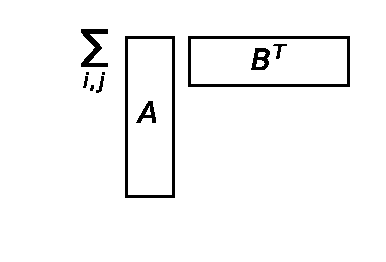
\includegraphics[width=130mm]{Results/normDifferenceFromUSVs.pdf}
%\caption[Exact norm of difference]{Visualising the calculation of the norm of a difference via SVD's}
%\label{fig:normDifferenceFromUSVs}
%\end{figure%}

%%%%%%%%%%%%%%%%%%%%%%%%%%%%%%%%%%%%%%%%%%
\section{Syntetic spatio-temporal fields}
\label{sec:Syntetic spatio-temporal fields}

For large data sets it is computational expensive to determine the level of autocorrelation. Hence, to compare our techniques and to establish a relation between performance and structure scale, we generate spatio-temporal fields, which resemble those often encountered in real-world applications, using \textit{Gaussian Random Fields} (GRF's). Their autocorrelation measurement is done with the well known Moran's $I$~\cite{Moran1950, Hubert1981, PySAL}.

\subsection{Gausssian Random Fields}
\label{sec:Autocorrelation/Gausssian Random Fields}
As simulated spatio-temporal fields, real-valued \textit{Gaussian Random Fields} (GRF's) are particularly useful because their structure scale can be captured in a single parameter. For such rotational invariant fields, the spectrum follows the power law described by $P(k) = c_{0} \, |\vec{k}|^{-\alpha}$ where $\vec{k}$ is the wavevector and~$\alpha$ the parameter which controls the level of autocorrelation. Figure~\ref{fig:GaussianRandomField} shows fields with various~$\alpha$'s.

\vspace{-2mm} % Remember
\begin{figure}[H]
\centering
\subfloat[$\alpha = 1$]{\label{fig:GaussianRandomFieldSize400Alpha1.pdf}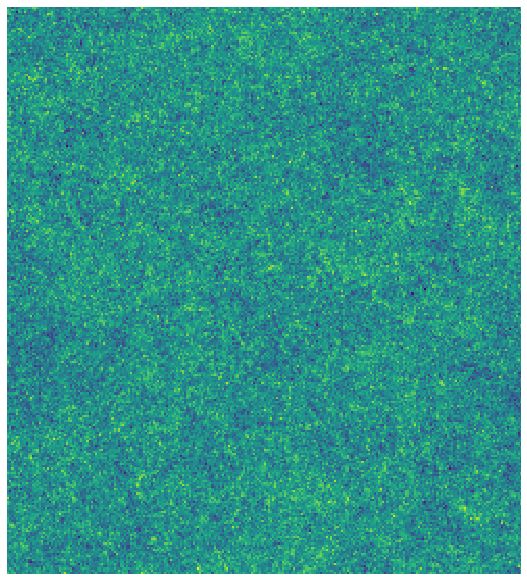
\includegraphics[scale=.38]{Results/GaussianRandomFieldSize400Alpha1.pdf}}
\hspace{8mm}
\subfloat[$\alpha = 3$]{\label{fig:GaussianRandomFieldSize400Alpha3.pdf}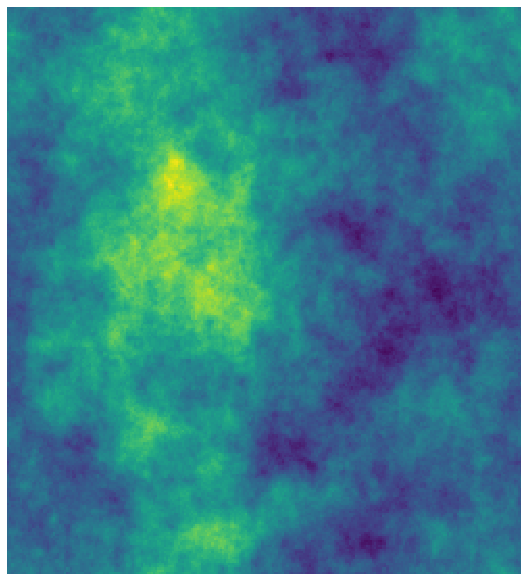
\includegraphics[scale=.38]{Results/GaussianRandomFieldSize400Alpha3.pdf}}
\hspace{8mm}
\subfloat[$\alpha = 5$]{\label{fig:GaussianRandomFieldSize400Alpha5.pdf}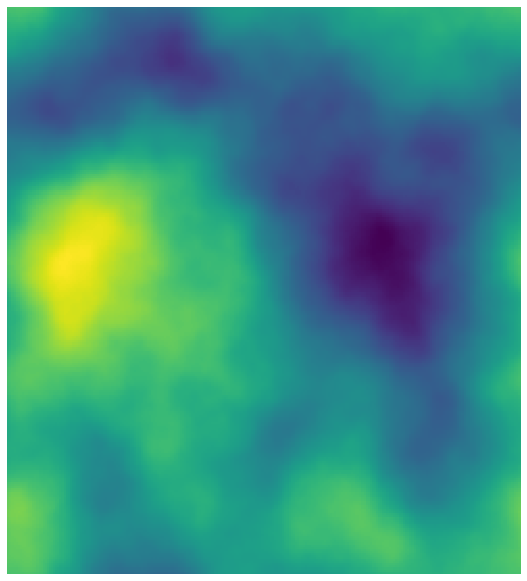
\includegraphics[scale=.38]{Results/GaussianRandomFieldSize400Alpha5.pdf}}
\caption{Gaussian Random Fields for various $\alpha$'s}
\label{fig:GaussianRandomField}
\end{figure}

Just as there is spatial autocorrelation, there is temporal autocorrelation, when the values of the field over the entire time period do not change drastically. In principle, there can be different levels of autocorrelation over time and over space. However, for simplicity, in this article we will use the same level of autocorrelation in all directions, determined by parameter~$\alpha$.

\subsection{Moran's $I$}
\label{sec:Autocorrelation/ Morans I}
In the geosciences, there are additional measures of spatial autocorrelation \cite{Eshel2011, Storch1999}. One frequently used is Moran's $I$~\cite{Moran1950, Hubert1981, PySAL}. Figure~\ref{fig:plotGammaAndMoransIAndBeta} shows the relationship between Moran's $I$, using a uniform kernel with a bandwidth equal to~$10$, and the $\alpha$ of our generated GRF's.

One can also devise an autocorrelation measure from the singular values of a dataset. Each singular value indicates the amount of variance explained by its associated mode. For fields with autocorrelation, the sorted list of singular values decays quickly. A power law can be fitted to this list, with an exponent which we call $\beta$.

\begin{figure}[H]
\centering
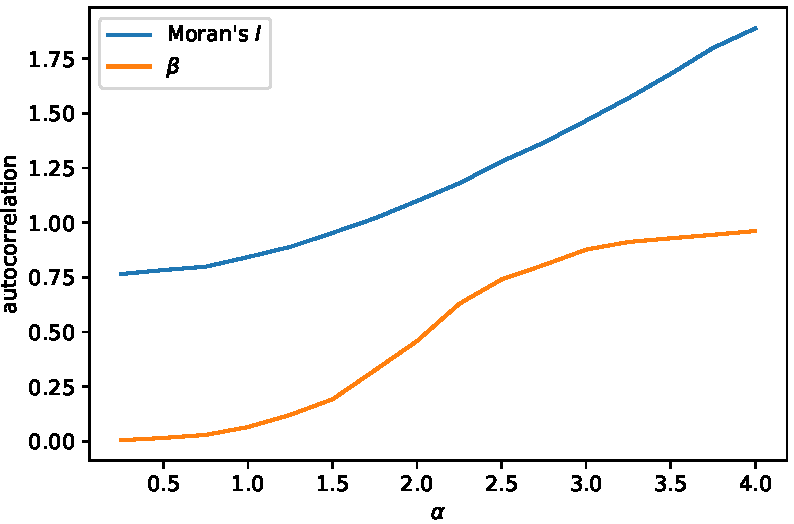
\includegraphics[width=80mm]{Results/plotMoransIAndBeta.pdf}
\caption[Various measures of autocorrelation]{Measures of autocorrelation as a function of $\alpha$}
\label{fig:plotGammaAndMoransIAndBeta}
\end{figure}

A high $\alpha$ implies a high Moran's $I$ and a high $\beta$, which, in turn, implies some singular values are close to zero. Therefore, spatial fields with high levels of autocorrelation are described by matrices which are approximate rank deficient. This allows for data reduction without losing much information.

%Much of the analysis here relies on knowledge of the level of autocorrelation, which may be difficult to determine for large datasets. The \textit{Jupyter Notebook} accompanying this article includes an algorithm which estimates Moran's $I$ based on a sample of gridpoints. This speeds up the calculation substantially compared with the full calculation. Further work could be placed into making this algorithm more professional and more user friendly. Additional areas of research include relaxing the assumption that the autocorrelation in the time direction is similar to that in the spatial directions. In fact, it is more realistic to allow for different levels of autocorrelation in all directions and to have a version of Moran's $I$ which can estimate these values.

%Furthermore, a warning about autocorrelation and standardisation. In MCA's, the timeseries of each spatial gridpoint is centred about its mean and in CCA's, each gridpoint is standardised. These operations destroy much of the spatial autocorrelation, as it can affect neighbouring cells differently. When researcher choose the coarsening technique, this should occur before any additional data processing steps.

\section{Methods}
\label{sec:Methods}
For very large datasets, which do not fit in \textit{RAM}-memory and are saved out-of-core, reading the data becomes a major factor in determining the speed of the analysis~\cite{Halko2011}. Size reduction can either enable data to be placed into internal memory or reduce the amount of bytes to be read from the local or remote storage. To achieve that we have selected SVD implementations to analyse large datasets efficiently by exploiting autocorrelation and rank deficiency. Additional methods exist, though the ones here cover three main benefits: the product SVD via QR decomposition provides an exact result, dimensionality reduction provides the best possible approximation for any level of reduction, while coarsening is an easy-to-implement method. 

For single fields, the choice between either exact SVD and approximate SVD depends whether it is applied to a rectangle or a square matrix. In case of a rectangle matrix, exact SVD via QR Decomposition is the best option, otherwise, approximate SVD via coarsening and dimensionality reduction is the best option. When the SVD is performed on the product of two matrices, the best course of action depends on whether the matrices are rectangular or square. For rectangle matrices, exact SVD via QR Decomposition is the best option while for square matrices an approximated answered is obtained via coarsening and dimensionality reduction. All these options are condensed into a decision tree to we help researcher identify situations where different SVD approaches are beneficial. Figure~\ref{fig:FlowDiagram} shows several options a researcher has when performing an SVD. 

\begin{figure}[H]
\centering
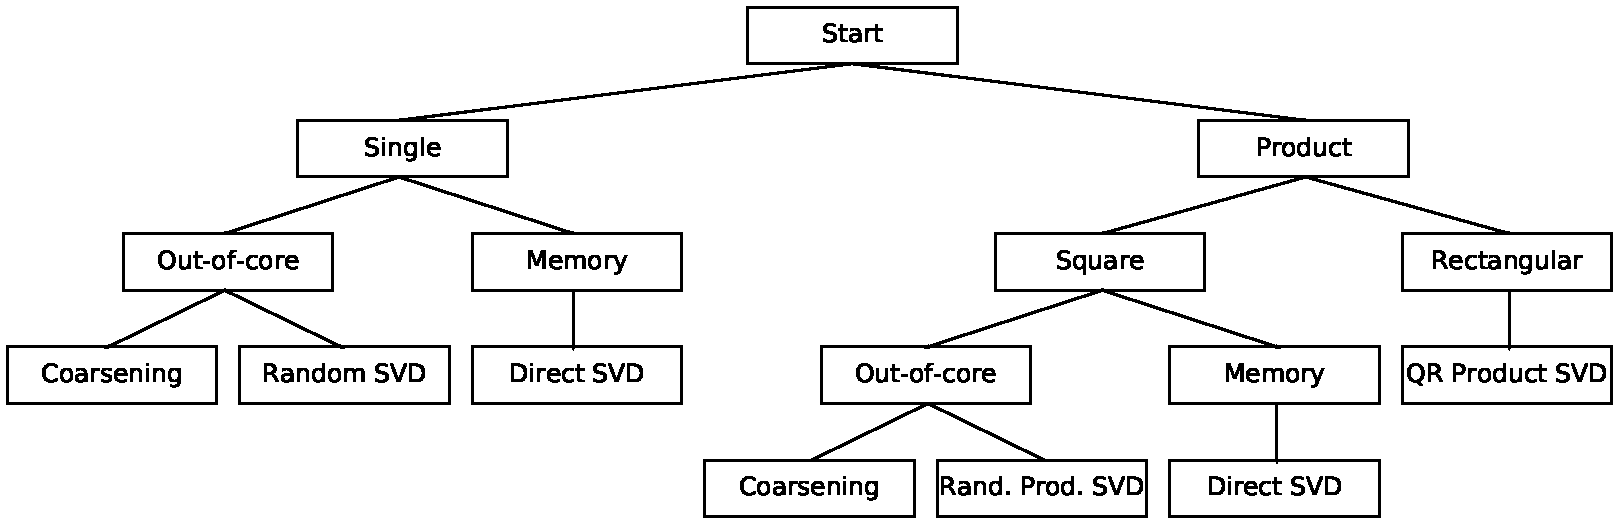
\includegraphics[width=\textwidth]{Results/FlowDiagram.pdf}
\caption{Decision tree describing the possible SVD techniques}
\label{fig:FlowDiagram}
\end{figure}


\subsection{Single fields}

\subsubsection{Exact SVD of a Singular Rectangular Matrix via QR Decomposition}

\subsubsection{Approximate SVD of a Single Matrix via Dimensionality Reduction}
\label{sec:Results/Approximate SVD of a Single Matrix via Dimensionality Reduction}
An alternative method of reducing the size of a matrix is via dimensionality reduction. During dimensionality reduction, the number of basis-vectors of a matrix is truncated to the~$l$ most important ones, similar to finding an $\epsilon$-rank approximation. Remember from section~\ref{sec:Introduction/Matrix Size and Rank} that matrices with low rank require less storage space and fewer flops for vector multiplications. A random algorithm exists which performs an approximate rank decomposition of a large matrix efficiently. This algorithm is reviewed extensively elsewhere, here we merely examine its performance on datasets with autocorrelation~\cite{Halko2011, Li2016}. One of its benefits is that this algorithm requires only a constant number of passes over the data. For large matrices, stored out-of-core, this reduces reading time. Additionally, the incurred error in the approximation can be made arbitrarily small by adjusting~$l$ and~$\epsilon$, giving the researcher full control over the balance between computation cost and accuracy.

\begin{figure}[H]
\centering
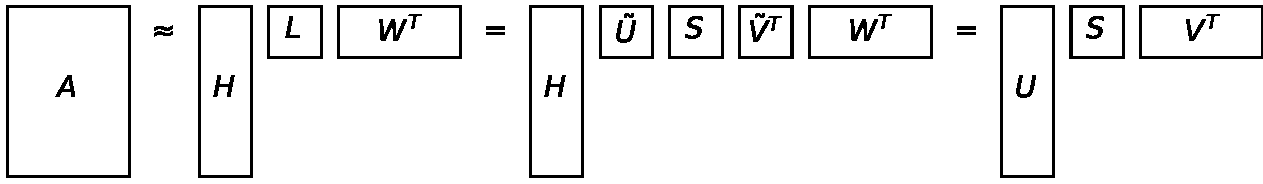
\includegraphics[width=100mm]{Results/reduceSizeRandomisedSquare.pdf}
\caption[Approximate randomised SVD]{Visualising the calculation of an approximate SVD via dimensionality reduction}
\label{fig:reduceSizeRandomisedSquare}
\end{figure}

Figure~\ref{fig:reduceSizeRandomisedSquare} depicts the calculation in this process, which first reduces the input matrix to a smaller square matrix of $l$~by~$l$. It also provides two projection matrices which rotate the rows and columns of this smaller matrix back as close as possible to the bases of the original input. Subsequently, the SVD is applied to the small $l$~by~$l$ matrix, which results in a fast and efficient approximation of the matrix's decomposition with an error of the order of the size of the largest truncated singular value~\cite{Martinsson2016, Halko2011}.

\subsubsection{Approximate SVD of a Single Matrix via Coarsening}
\label{sec:Results/Approximate SVD of a Single Matrix via Coarsening}
When a spatial field has large scale structure, the values of neighbouring cells do not change drastically. Perhaps these cells can be aggregated together to produce a smaller dataset which still faithfully describes the original field. Here, we coarsen two dimensional GRF's. Figure~\ref{fig:plotSingleSpatialFieldViaCoarsening} shows the error in a coarsening process for matrices of various~$\alpha$'s and for different coarsening window sizes. The error is determined as the norm of the difference between the original matrix and the coarsened version, divided by the norm of the original~\cite{Bogaardt2018}. Other measures of similarity could have been used, such as the correlation between the two datasets, but this is left for future research. Note that coarsening a two dimensional field at level 5 reduces the dataset by $25$ times. For fields with high autocorrelation, e.g. $\alpha=3$, the coarsened version differs by less than~$10\%$ from the original.

\begin{figure}[H]
\centering
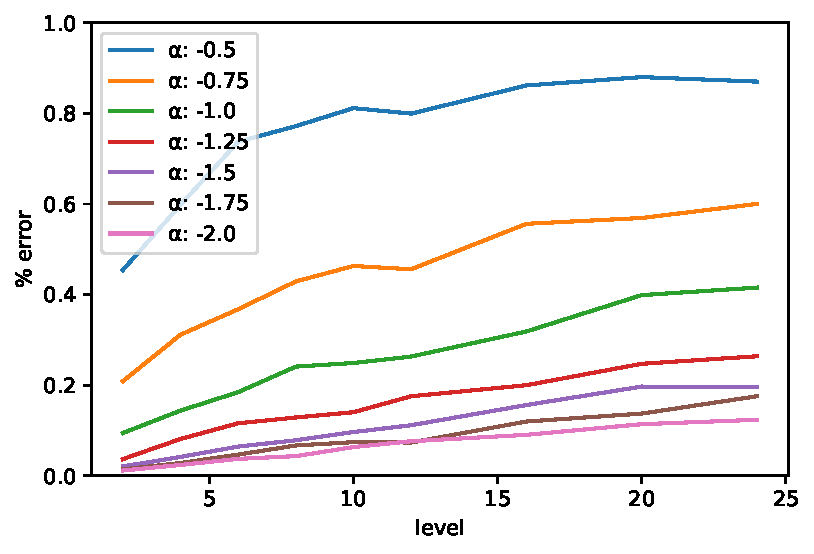
\includegraphics[width=80mm]{Results/plotSingleSpatialFieldViaCoarsening.pdf}
\caption[Error after coarsening]{Error in the SVD of a coarsened spatial field for various $\alpha$'s}
\label{fig:plotSingleSpatialFieldViaCoarsening}
\end{figure}

The calculations in the accompanying \textit{Jupyter Notebook} show that the errors induced by the randomised SVD procedure are very small, even for high levels of reduction~\cite{Bogaardt2018}. The technique performs much better than coarsening. The coarsening procedure has several advantages though. For one, it is intuitive and the results are easy to interpret. It is also trivial to implement. Additionally, different coarsening levels can be applied to different directions. This is especially advantages when directions have different levels of autocorrelation or are recorded at different resolutions. Finally, the predictions of figure~\ref{fig:plotSingleSpatialFieldViaCoarsening} can help researchers determine at what resolution to gather their data in the first place. In domains were satellite data is used, datasets are often not very detailed because the imaging resolution is low. Unlike local analyses of developed countries, where high resolution data is becoming more accessible, for continental or global analyses, coarse spatial resolution data may simply be the only option.


\subsection{Product of two matrices}

\subsubsection{Exact Product SVD of Rectangular Matrices via QR Decomposition}
\label{sec:Results/Exact Product SVD of Rectangular Matrices via QR Decomposition}
In an MCA and CCA, an SVD is performed on the product of two spatio-temporal fields to find patterns which occur frequently and simultaneously~\cite{Eshel2011, Storch1999}. For highly rectangular datasets, when there are many spatial gridpoints but few temporal samples, the resulting cross-covariance matrix is inefficiently large and obviously rank deficient. Performing a rank decomposition on each dataset before multiplying them allows the SVD to be calculated in an efficient manner~\cite{Chan1982, Tygert2017}. Figure~\ref{fig:qrProductSVD} depicts the calculation in this technique. Using the QR decomposition, the input datasets are first transformed into two square, full rank matrices together with rectangular orthonormal basis vectors. The SVD is then performed on the product of the small, square matrices, giving a mathematically identical result to the full SVD while never forming an unnecessarily large, intermediate matrix.

\begin{figure}[H]
\centering
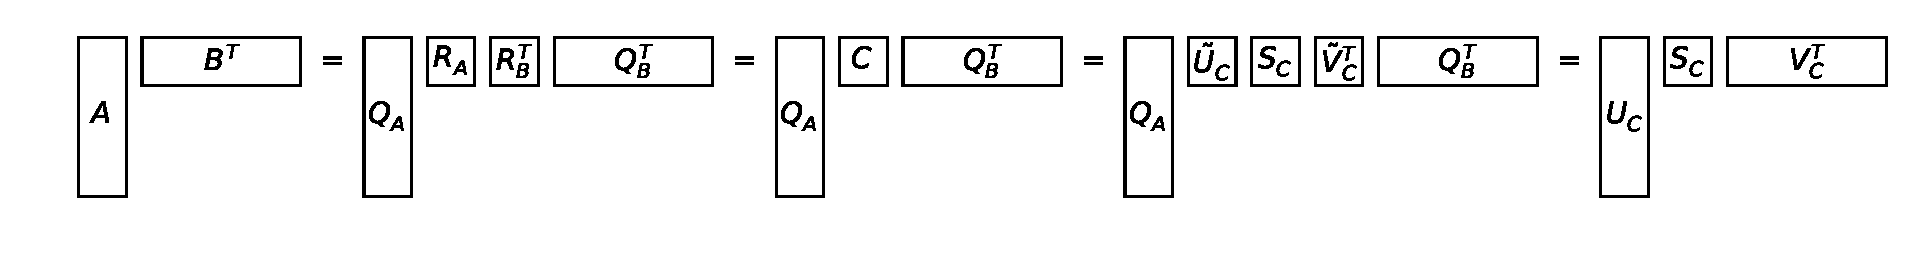
\includegraphics[width=\textwidth]{Results/qrProductSVD.pdf}
\caption[Exact SVD via QR decomposition]{Visualising the calculation of the exact SVD of a product via QR decomposition}
\label{fig:qrProductSVD}
\end{figure}

\subsubsection{Approximate Product SVD of Square Matrices via Dimensionality Reduction}
\label{sec:Results/Approximate Product SVD of Square Matrices via Dimensionality Reduction}
The randomised dimensionality reduction process can be applied to two spatio-temporal fields before they are multiplied into the cross-covariance matrix. Similar to the QR decomposition of section~\ref{sec:Results/Exact Product SVD of Rectangular Matrices via QR Decomposition}, it has the advantage that the SVD is applied to a small $l$~by~$l$ matrix. This calculation is visualised in figure~\ref{fig:randomisedSquareProductSVD}. In the first step, the input datasets are decomposed using an algorithm which is reviewed extensively elsewhere~\cite{Halko2011, Li2016}. Subsequently, the SVD is performed on the small, inner matrix.

\begin{figure}[H]
\centering
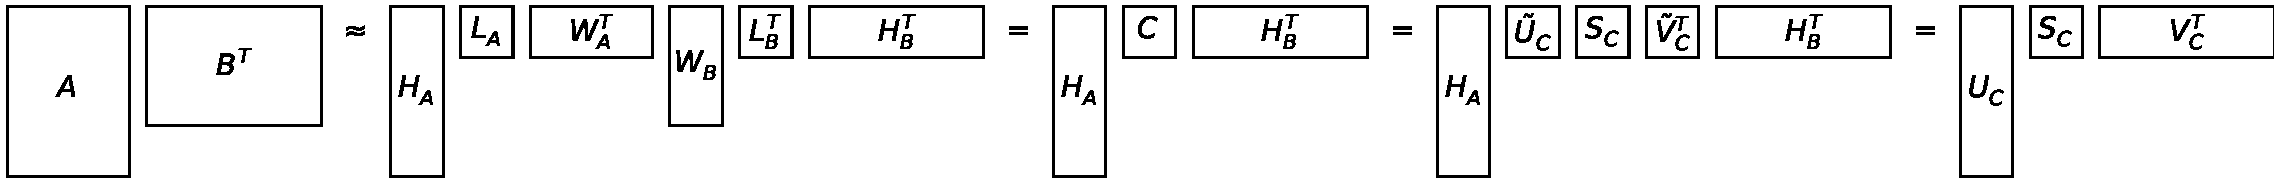
\includegraphics[width=\textwidth]{Results/randomisedSquareProductSVD.pdf}
\caption[Approximate product SVD]{Visualising the calculation of an approximate SVD for the product of two fields using dimensionality reduction}
\label{fig:randomisedSquareProductSVD}
\end{figure}

After generating various GRF's, the reduced cross-covariance matrix is compared with the original. Figure~\ref{fig:plotRandomisedSizeReducedMatrixProduct} shows that the results are quite bad for fields with a small $\alpha$, but high levels of autocorrelation allow for substantial savings in computation time without incurring much error. When performing an MCA or CCA on a spatio-temporal field, the spatial directions are flattened and some of the spatial autocorrelation is lost. This partially explains why the error is substantial for low $\alpha$. Again, we performed our analysis with two generated fields which correlated to some degree. How this correlation influences the amount of error after dimensionality reduction is left for further research.

\begin{figure}[H]
\centering
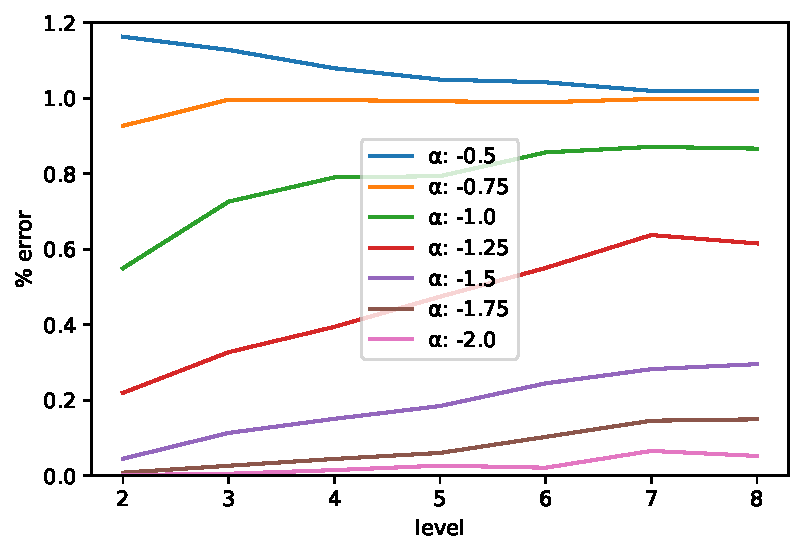
\includegraphics[width=80mm]{Results/plotRandomisedSizeReducedMatrixProduct.pdf}
\caption[Error after reduction]{Error in the SVD of the product of two reduced fields for various $\alpha$'s}
\label{fig:plotRandomisedSizeReducedMatrixProduct}
\end{figure}

The reduction of the number of dimensions of each input dataset before an MCA or CCA is actually advised by some researchers, as a method to filter out noise~\cite{Barnett1987}. Especially when the number of temporal samples is small, outliers and random fluctuations could affect the result~\cite{Bretherton1992}. This is because any statistical analysis will choose its regression-coefficients so as to optimize the fit. It may occur that two noise-vectors in the two fields coincidentally covary and show up as dominant modes. Prefiltering can alleviate this risk.

\subsubsection{Approximate Product SVD of Square Matrices via Coarsening}
\label{sec:Results/Approximate Product SVD of Square Matrices via Coarsening}

In real-world applications, researchers often wants to find the relation between two fields. Analyses such as the MCA and CCA, discussed in section~\ref{sec:Introduction/Decision Tree}, rely on performing an SVD of the product matrix of two spatio-temporal fields. Take the input datasets with the various spatial gridpoints as rows and the sample of recorded values over time as columns, multiplying these gives the cross-covariance matrix. While section~\ref{sec:Results/Approximate SVD of a Single Matrix via Coarsening} dealt with coarsening a single spatial field, we can also coarsen two fields before analysing their cross-covariance matrix. Figure~\ref{fig:plotProductSpatialTemporalFieldsViaCoarsening} shows the percentage error for various generated spatio-temporal fields. Note that only the spatial directions are coarsened in our calculation. This is because the time direction gets consumed in the matrix product of the MCA or CCA and coarsening it will not speed up the SVD. Coarsening two spatial directions means each field is reduced by the square of the coarsening level, while the cross-covariance matrix is reduced by this level to the power~$4$. As a result, the typical error in this product is larger than for the single field, though the speed up is also substantial. Clearly, the level of autocorrelation plays an important part, with larger~$\alpha$'s leading to less error. Preliminary work shows the amount of error also depends on the similarity between the two spatio-temporal fields, though we leave deeper investigation of this aspect for further research. 

\begin{figure}[H]
\centering
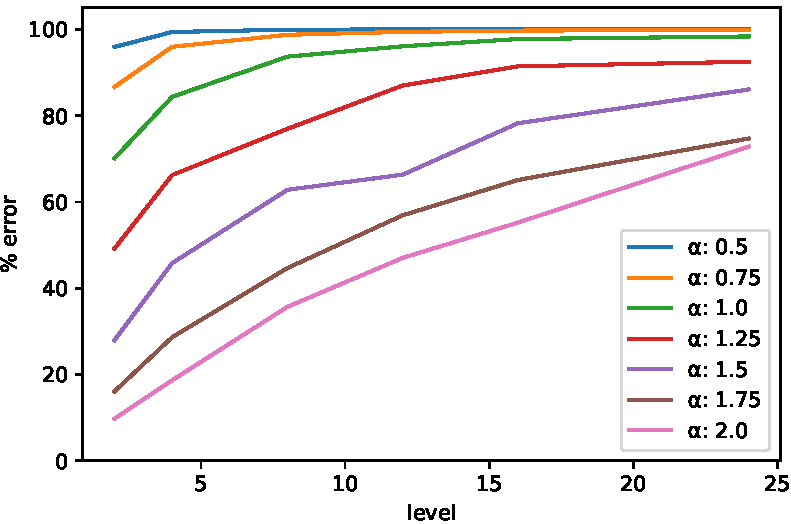
\includegraphics[width=80mm]{Results/plotProductSpatialTemporalFieldsViaCoarsening.pdf}
\caption[Error after coarsening]{Error in the SVD of the product of two coarsened fields for various $\alpha$'s}
\label{fig:plotProductSpatialTemporalFieldsViaCoarsening}
\end{figure}

\section{Results}
In this section through three use cases...

\subsection{Case Study of an SVD of a Single Matrix}
\label{sec:Results/Case Study of an SVD of a Single Matrix}

Coarsening and dimensionality reduction are particularly useful for spatial fields with high levels of autocorrelation. As an example of this, we examine humidity and cloud cover data from the ERA5 datasets for a single time period. ERA5 is an atmospheric reanalysis of the global climate using high spatial resolution forecasts, produced by combining models with observations~\cite{Dee2011}. It contains estimates of atmospheric parameters such as air temperature, pressure and wind at different altitudes.

Clearly, the ERA5 humidity and cloud cover fields are not GRF's. Nonetheless, we can get an idea of the accuracy of an SVD after data reduction if we estimate the levels of autocorrelation. This can verify whether simulated GRF's are reasonable representations of real-world datasets. The humidity field has a Moran's $I \approx 0.98$, while the cloud cover data shows less structure with a Moran's $I \approx 0.82$. The estimations for~$\alpha$ were unreliable, though figure~\ref{fig:plotGammaAndMoransIAndBeta} can help us translate the measures and suggests the fields are equivalent to GRF's with an $\alpha \sim 3.5$ and $\alpha \sim 2.5$, respectively.

The coarsening predictions of figure~\ref{fig:plotSingleSpatialFieldViaCoarsening} indicate the first field is expected to incur errors around a few percent for size reductions between~$2$ and~$8$, while for the second field we should see errors between~$5\%$ and~$15\%$. The calculations in the \textit{Jupyter Notebook} in the supplementary material show that this prediction is fairly accurate, perhaps slightly pessimistic. For the dimensionality reduction, the errors are, as expected, very small; below $1\%$. If a researcher cares most about performance, dimensionality reduction is the best option.


\subsection{Case Study of a Product SVD of Rectangular Matrices}
\label{sec:Results/Case Study of a Product SVD of Rectangular Matrices}

Let's apply the QR decomposition technique to phenological datasets. Phenology is the science that studies recurring biological events such as leafing and blooming as well as their causes and variations in space and time. Spatio-temporal fields of remotely sensed images can be used to derive various phenological metrics. One of these metrics is the so-called \textit{Start of Season} (SOS), which indicates the beginning of photosynthetic activity in plants. In this section, we use a SOS field of the US, made by processing time series of the \textit{Advanced Very High Resolution Radiometer} (AVHRR) sensor~\cite{Reed1994}. Additionally, we use the \textit{Extended Spring Indices} (SI-x), which are a suite of models that transform daily temperatures into consistent phenological metrics~\cite{Schwartz2013}. In particular, we take a version of the Bloom index which was recently generated for the US by adapting the SI-x models to a cloud computing environment~\cite{Izquierdo2015}. Both datasets span from $1989$ to $2014$ and have a $1\text{km}^2$ spatial resolution, meaning there are far fewer time periods than spatial gridpoints giving highly rectangular matrices. In fact, each dataset contains $30$ million rows and $26$ columns and is about $3.2$GB large. Their cross-covariance would be $30$ million rows by $30$ million columns and about $3.7$PB in size. Luckily, this product matrix need not be created to perform the SVD.

For the SVD via QR decomposition, the autocorrelation measures have no effect because this technique provides a mathematically exact result. Indeed, the \textit{Jupyter Notebook} in the supplementary material, as well as work being prepared for publication, shows that this technique provides the full SVD of the cross-covariance matrix for these datasets in a matter of seconds, without ever exceeding the \textit{RAM}-memory~\cite{Bogaardt2018, ZuritaMilla2018}.

\subsection{Case Study of a Product SVD of Square Matrices}
\label{sec:Results/Case Study of a Product SVD of Square Matrices}

The JRA55 data is an atmosphere reanalysis product which includes quantities such as humidity, pressure and temperature~\cite{Kobayashi2015}. Recently, these quantities were used to determine the total meridional energy transport and latent heat, measures important to understand the global climate~\cite{Liu2018}. As an example of our reduction techniques for matrix products, we are using a Mercator projection of the energy transport and latent heat, recorded monthly from 1979 to 2015. Although the spatially flattened matrices are not completely square, their high resolution in the time direction make them substantially less rectangular than the phenology data from section~\ref{sec:Results/Case Study of a Product SVD of Rectangular Matrices}. Therefore, this serves as a good use case for the coarsening and dimensionality reduction techniques for a square product SVD.

The energy field has a Moran's $I \approx 0.93$, while the latent heat field has a Moran's $I \approx 0.86$. The estimations for~$\alpha$ were unreliable, though figure~\ref{fig:plotGammaAndMoransIAndBeta} can help us translate the measures and suggests the fields are equivalent to GRF's with an $\alpha \sim 3.0$ and $\alpha \sim 2.5$, respectively. The analyses of section~\ref{sec:Results/Approximate Product SVD of Square Matrices via Coarsening} and of section~\ref{sec:Results/Approximate Product SVD of Square Matrices via Dimensionality Reduction} showed that, for such~$\alpha$ levels, the errors should be quite high. In contrast, we found that coarsening the fields before applying an SVD on their product merely resulted in an error between $8\%$ and $16\%$. For the dimensionality reduction technique, as well, the predictions overstated the observed error, which were around a few percent, even for high levels of size reduction. 


%%%%%%%%%%%%%%%%%%%%%%%%%%%%%%%%%%%%%%%%%%
\section{Discussion}


Unlike the coarsening procedure, the dimensionality reduction is not applied on each spatial field for each time period, but rather on the entire spatially flattened timeseries. Therefore, the level of spatial autocorrelation may not be as important as the level of temporal autocorrelation. Further work can examine how to apply the reduction to the spatial part of the spatio-temporal fields, before it is flattened. Alternative solutions, which retain the spatial structure, may include 3D tensor operations such as \textit{Higher-Order Singular Value Decomposition} (HOSVD)~\cite{Tucker1964}.

This requires knowledge of the precision of the data gathering equipment and setting a desired level of accuracy for the final output.
\subsection{Summary}
\label{sec:Discussion/Summary}

In summary, randomised dimensionality reduction works best for datasets which are too large for internal memory [RG: What happens when they do not fit in memory? Is there and experiment that shows that?]. It requires only a constant number of passes over the data, which decreases storage reading time. It also allows the researcher to balance computation cost with accuracy, by tuning the algorithm's parameters. Performing analyses at a coarse level can be beneficial when data collection is difficult and provides an intuitive and easy-to-implement alternative. These techniques require at least some autocorrelation in the fields, which results in rank deficient datasets. In general, rank decompositions can speed up calculations by splitting datasets into smaller matrices of full rank. For rectangular matrices, this can give a mathematically exact result. Once the analysis is performed on the smaller matrix, the output can be rotated back to the original bases, saving memory usage and computation time.
\\

%%%%%%%%%%%%%%%%%%%%%%%%%%%%%%%%%%%%%%%%%%
%\section{Conclusions}

%This section is not mandatory, but can be added to the manuscript if the discussion is unusually long or complex.

%%%%%%%%%%%%%%%%%%%%%%%%%%%%%%%%%%%%%%%%%%
%\section{Patents}
%This section is not mandatory, but may be added if there are patents resulting from the work reported in this manuscript.

%%%%%%%%%%%%%%%%%%%%%%%%%%%%%%%%%%%%%%%%%%
\vspace{6pt} 

%%%%%%%%%%%%%%%%%%%%%%%%%%%%%%%%%%%%%%%%%%
\authorcontributions{Conceptualization, R.Z.; Methodology, L.B.; Software, L.B.; Validation, R.G., R.Z. and E.I.; Formal Analysis, L.B.; Investigation, L.B.; Resources, R.G., R.Z. and E.I.; Data Curation, R.G., R.Z. and E.I.; Writing—Original Draft Preparation, L.B.; Writing—Review \& Editing, R.G., R.Z. and E.I.; Visualization, L.B.; Supervision, R.G. and R.Z.; Project Administration, R.G.; Funding Acquisition, R.Z.}

%%%%%%%%%%%%%%%%%%%%%%%%%%%%%%%%%%%%%%%%%%
\funding{This research was funded by the Nederlandse Organisatie voor Wetenschappelijk Onderzoek (NWO).}

%%%%%%%%%%%%%%%%%%%%%%%%%%%%%%%%%%%%%%%%%%
%\acknowledgments{In this section you can acknowledge any support given which is not covered by the author contribution or funding sections. This may include administrative and technical support, or donations in kind (e.g. materials used for experiments).}

%%%%%%%%%%%%%%%%%%%%%%%%%%%%%%%%%%%%%%%%%%
\conflictsofinterest{The authors declare no conflict of interest. The founding sponsors had no role in the design of the study; in the collection, analyses, or interpretation of data; in the writing of the manuscript, and in the decision to publish the results.} 

%%%%%%%%%%%%%%%%%%%%%%%%%%%%%%%%%%%%%%%%%%
%% optional
\abbreviations{The following abbreviations are used in this manuscript:\\

\noindent 
\begin{tabular}{@{}ll}
SVD & Singular value decomposition\\
GRF & Gaussian random field\\
PC & Principle component\\
EOF & Empirical orthogonal function\\
SOS & Start of season\\
SI-x & Extended spring indices\\
AVHRR & Advanced very-high-resolution radiometer\\
ERA5 & European fifth generation reanalysis\\
JRA55 & Japanese 55-year reanalysis\\
HOSVD & Higher-order singular value decomposition
\end{tabular}}

%%%%%%%%%%%%%%%%%%%%%%%%%%%%%%%%%%%%%%%%%%
%=====================================
% References, variant B: external bibliography
%=====================================
\externalbibliography{yes}
\bibliography{Bibliography}

%%%%%%%%%%%%%%%%%%%%%%%%%%%%%%%%%%%%%%%%%%
\end{document}

